% Collective Intelligence 2017 LaTeX format
% Adapted from ACM Large format by Walter S. Lasecki
%
%
% Steps to compile: latex, bibtex, latex, latex
%
\documentclass[prodmode,acmtap]{ci2018}
\usepackage{subcaption}
\captionsetup{compatibility=false}
\graphicspath{{images/}}

% Metadata Information
\acmVolume{2}
\acmNumber{3}
\acmArticle{1}
\articleSeq{1}
\acmYear{2010}
\acmMonth{5}

% Package to generate and customize Algorithm as per ACM style
\usepackage[ruled]{algorithm2e}
\SetAlFnt{\algofont}
\SetAlCapFnt{\algofont}
\SetAlCapNameFnt{\algofont}
\SetAlCapHSkip{0pt}
\IncMargin{-\parindent}
\renewcommand{\algorithmcfname}{ALGORITHM}

% Page heads
\markboth{R. Engelhardt, J. Stærk-Østergaard and V.F. Hendricks}{The Wisdom and Manipulability of Threads}

% Title portion
\title{The Wisdom and Manipulability of Threads}
\author{ROBIN ENGELHARDT, JACOB STÆRK-ØSTERGAARD and VINCENT FELLA HENDRICKS
 \affil{University of Copenhagen}
}
% NOTE! Affiliations placed here should be for the institution where the
%       BULK of the research was done. If the author has gone to a new
%       institution, before publication, the (above) affiliation should NOT be changed.
%       The authors 'current' address may be given in the "Author's addresses:" block (below).
%       So for example, Mr. Fogarty, the bulk of the research was done at UIUC, and he is
%       currently affiliated with NASA.

\begin{abstract}
Intentionally left blank.
\end{abstract}


% At a minimum you need to supply the author names, year and a title.
% IMPORTANT:
% Full first names whenever they are known, surname last, followed by a period.
% In the case of two authors, 'and' is placed between them.
% In the case of three or more authors, the serial comma is used, that is, all author names
% except the last one but including the penultimate author's name are followed by a comma,
% and then 'and' is placed before the final author's name.
% If only first and middle initials are known, then each initial
% is followed by a period and they are separated by a space.
% The remaining information (journal title, volume, article number, date, etc.) is 'auto-generated'.



\begin{document}

\maketitle

% PS: BUG in template means that all multiple citations in \cite{...} should be without spaces.

% Head 1
\section{Introduction}

Social information in the form of opinions and judgments by other people is sampled sequentially. We read the news, hear rumors, listen to debates on TV, and flip through comments on social media platforms and blogs. These activities inform us and influence our decisions, but researchers still debate the conditions under which these types of social information help us make better decisions \cite{woolley2010evidence,gurccay2015power,becker2017network,jayles2017social}, lead us astray \cite{lorenz2011social,minson2012cost,le2018endogenous}, or just make us confused at a higher level \cite{salganik2006experimental}. 

Collective estimates of a diverse group of people can outperform the majority of its members because any random confusion at the individual level is likely to average out and let the most accurate estimate prevail \cite{galton1907vox,surowiecki2005wisdom}. Then again, confusion is not always randomly scattered around the truth. Systematic biases in individual perception may create measurable disruptions in the wisdom of crowds \cite{izard2008calibrating,kao2018counteracting}. Social information can add to those biases and create echo chambers, bandwagoning, herd behavior \cite{bikhchandani1992theory,bakshy2015exposure,banerjee1992simple}, and various belief misattributions \cite{katz1931students,ross1977false,lee2019homophily}, which uphold harmful social practices despite being rejected by a majority of people. Social information may also have been intentionally filtered or manipulated in various ways, for instance through group pressure, algorithmic filtering \cite{pariser2011filter}, false cues \cite{muchnik2013social,hanson1996hits}, or simply by plain misinformation \cite{hendricks2018reality}, often with highly detrimental consequences for our economy and our health.

Observational data of decision-making processes is acutely sensitive to the social context in which people find themselves. Thus, researchers find it difficult to separate observational data into its social and individual components. How may we know how much weight an individual puts on her own ‘independent’ estimate relative to the weight put on the estimates by others? Randomized experimental studies have attempted to solve this problem by first letting participants make a magnitude estimate of an object without social information (\textit{ex ante}), and subsequently ask them to revise their estimate after having received information about other people’s estimates of that object (\textit{ex post}) \cite{becker2017network,jayles2017social,lorenz2011social,mavrodiev2013quantifying}. This double elicitation paradigm presumes that people change their mind because of the social information they have received. Other studies, however, have shown that people routinely can change their mind all by themselves, and that it may be more correct to assume an `inner crowd' in the sense that people sample randomly from a probability distribution in their own mind \cite{vul2008measuring,herzog2014harnessing}. Such a psychological mechanism (and others such as hedging strategies due to anticipated regrets \cite{bell1982regret}, and/or disappointments \cite{loomes1986disappointment}) make it difficult to differentiate accurately between `inner' samples and `outer' influences, and it may be desirable to develop an alternative model framework that is able infer the extend of individual bias and social influence from a single task. 

We propose to use probabilistic gaussian mixture models (GMMs) since they have two properties that are highly valuable in the context of free response elicitation tasks. First, GMMs are comprised of several Gaussians which fit well to the often highly right-skewed and long-tailed distributions of estimates. Second, GMMs associate an uncertainty measure to each data point, telling us how much an estimate may be associated to a sub-population of people who are influenced in a certain way by the social information, without having any prior identity information about sub-populations in the data set. 

%In real life people rarely estimate twice and rarely have access to all the relevant social information. So if we wish to get closer to a naturalistic experimental setting, we should create situations in which people see only a small fraction of the social information out there. In addition, social information is rarely sampled at random. People typically collect social information from certain people, in certain places and in certain time intervals, for instance via a discussion thread, in user reviews, or in similar successive pronouncements after which they make up their mind. The effects of the clustered, sparse, and sequential nature of social information on decision-making have not been investigated systematically before and may turn out to have a substantial impact on both individual decision-making and on the accuracy of the crowd. 

\section{Thread Medians}

Using a cascade design that emulates succesive decision-making, we investigate experimentally the collective accuracy and manipulability of threads. The data was collected from 7,814 participants playing a dot-guessing game \cite{horton2010dot} on Amazon Mechanical Turk, where each participant successively estimated the number of visible dots $d \in \{55,148,403,1097\}$ in various images, while seeing $v \in \{0,1,3,9\}$ preceding estimates (historical threads). An additional 3,934 participants were shown the same images while seeing the $v \in \{1,3,9\}$ \textit{highest} estimates made so far (manipulated threads). 

\begin{figure*}[!h]
\centering
	\begin{subfigure}[t]{.46\linewidth}
		\centering
		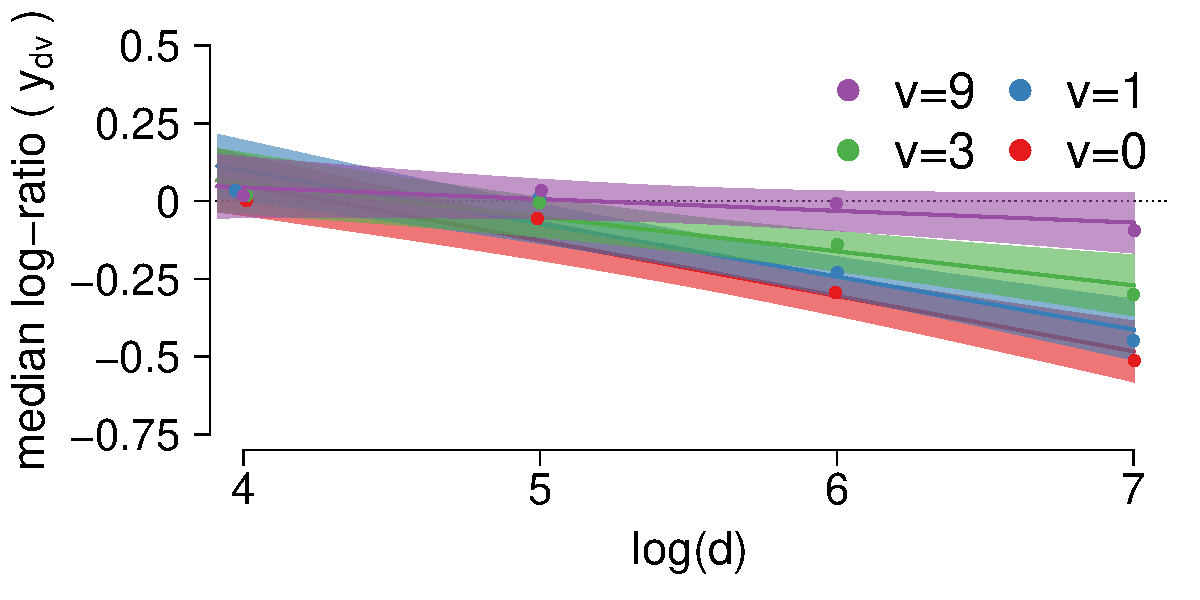
\includegraphics[width=1\linewidth]{med_confidence_h.pdf}	
		\caption{\footnotesize Historical threads.}
		\label{fig: median confidence bounds - historic}
	\end{subfigure}
	\begin{subfigure}[t]{.46\linewidth}
		\centering
		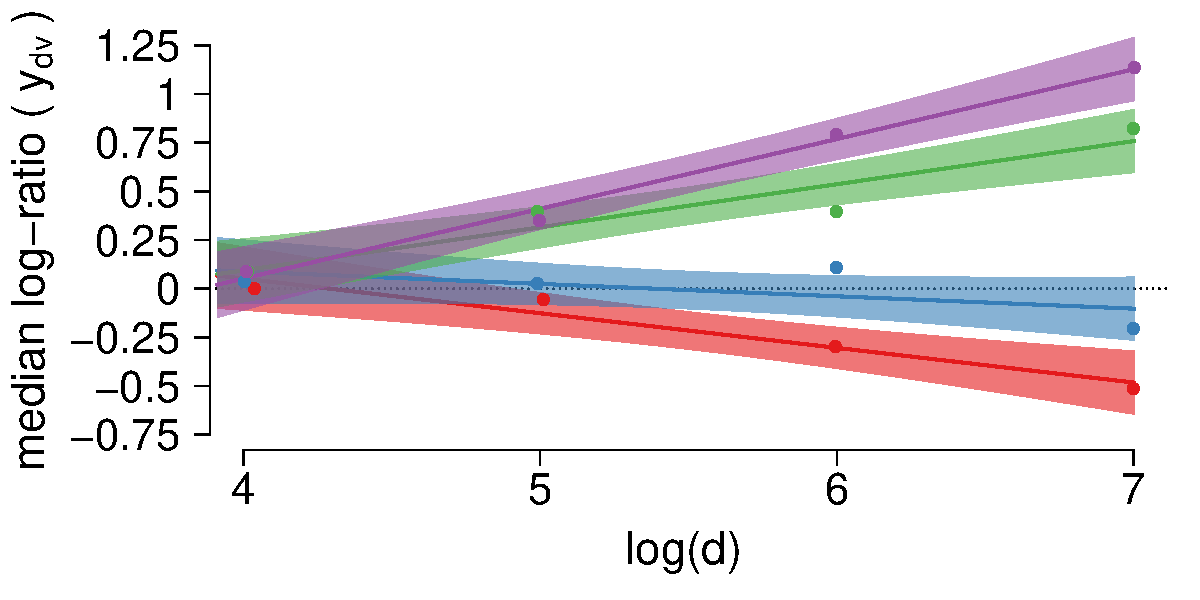
\includegraphics[width=1\linewidth]{med_confidence_m.pdf}		
		\caption{\footnotesize Manipulated threads.}
		\label{fig: median confidence bounds - manipulated}
	\end{subfigure}
	\caption{Relationship between median log-ratio $y_{dv}$ and $\log(d)$ with 95\% confidence bounds (shaded areas). The colors represent the four settings on number of visible estimates. There is a clear relation between number of dots and number of visible estimates in both thread types, but it is more pronounced for the manipulated series. The red lines corresponding to the control groups with $v=0$ are the same in both plots.}
	\label{fig: median confidence bounds}
\end{figure*}

We compare the log-ratio of the individual thread medians, $y_{dv}=\log(M_{(d,v)}/d)$, using a linear normal model to quantify differences between threads in terms of $\log(d)$ and $v$, the latter as a categorical variable. Figure \ref{fig: median confidence bounds - historic} shows that the collective performance for historical threads declines significantly with increasing task difficulty (higher $d$), but improves when the social information is substantial (high $v$). In contrast to \cite{lorenz2011social} and in accordance with \cite{gurccay2015power,becker2017network}, this finding supports the claim that crowds indeed may become wise under (pristine) social influence. It should be noted, however, that the overlapping confidence intervals reveal where thread performances are comparable. The combination of the negative effects of task difficulty and the positive effects of social information are only discernible in situations where people have hard problems to solve and at the same time have plenty of social information available.

For the manipulated series, Fig.\ref{fig: median confidence bounds - manipulated}, the manipulation gives a large positive bias for $v=3,9$ which increases with $d$, implying that when a task becomes more demanding, the amount of manipulated social information has a detrimental impact on thread performance.

\section{Social Influence}

Figure \ref{fig: social influence} displays the effect of social information, obtained by fitting a GMM to each thread using the geometric mean of visible estimates as a proxy for the available social information. The effect of social information on each participant is given by $\tilde{\beta}$, the weighted average of the individual states of the GMM, where a high value ($\tilde{\beta}>0.6$, blue color) implies a large effect, a low value ($\tilde{\beta}\approx 0$, red color) implies little or no effect and a medium value ($\tilde{\beta} \approx 0.4$, green color) suggests a compromise between the two extremes.

\begin{figure*}[!ht]
	\centering
	\begin{subfigure}[t]{.44\linewidth}
		\centering
		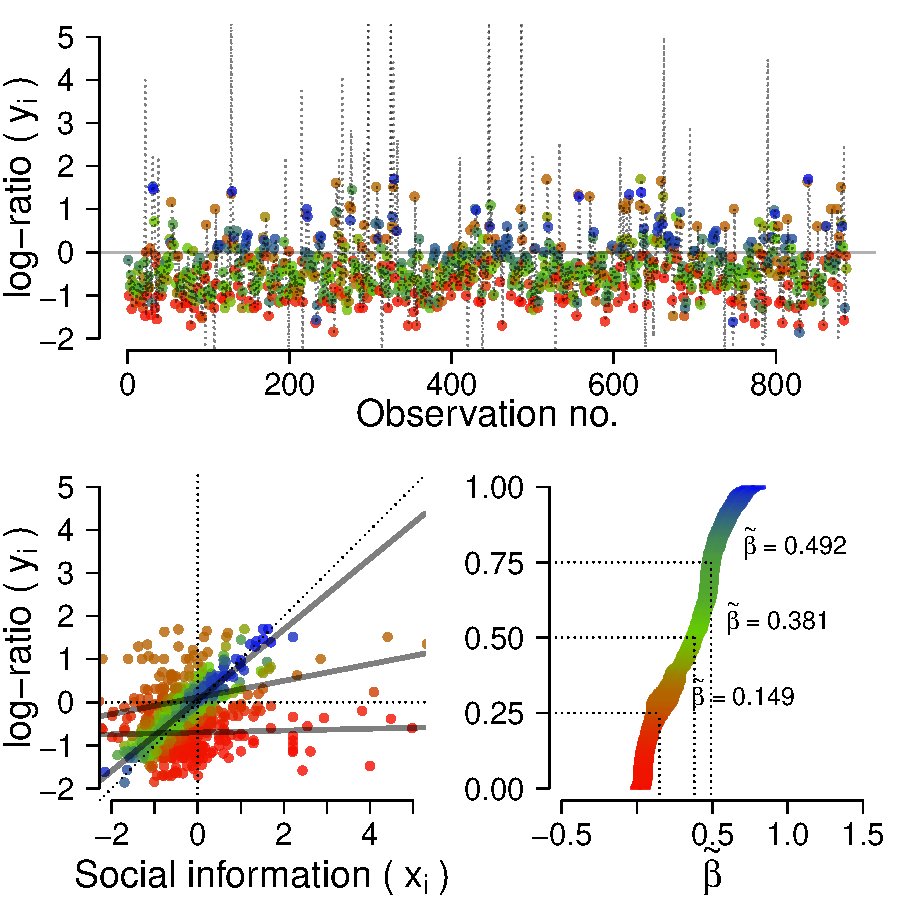
\includegraphics[width=1\linewidth]{h10971.pdf}
		\caption{\footnotesize Historical thread with $d=1097$ and $v=1$}
		\label{fig: h d=1097, v=1}
	\end{subfigure}
	\begin{subfigure}[t]{.44\linewidth}
		\centering
		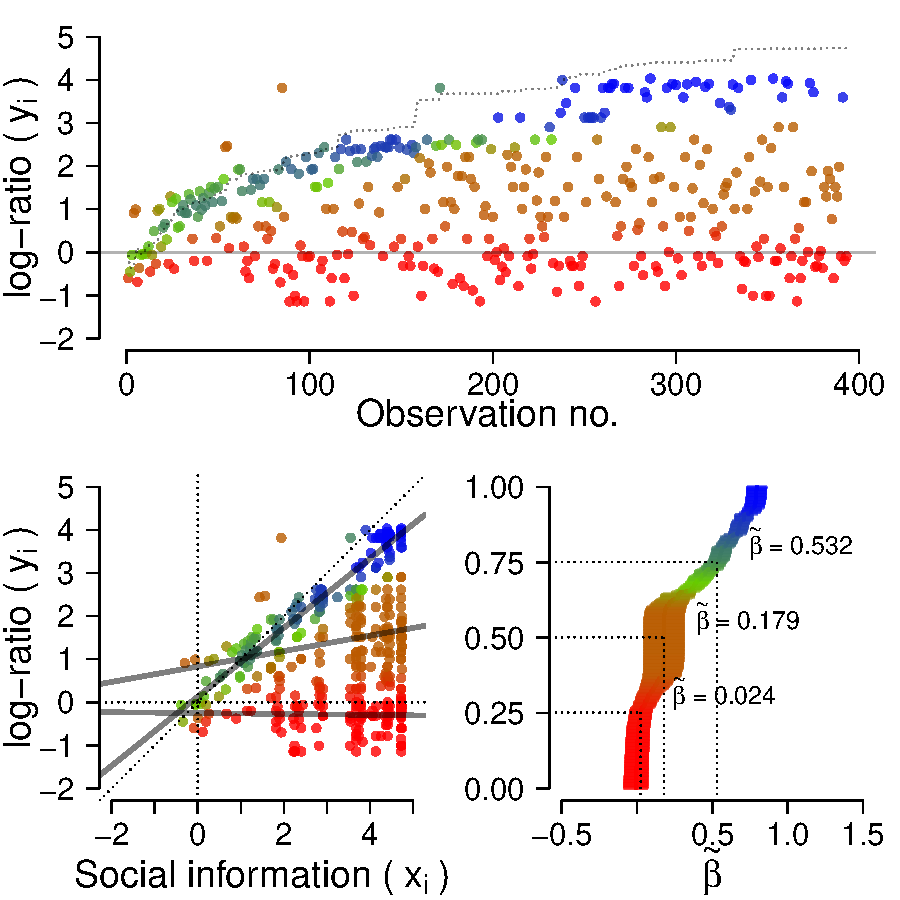
\includegraphics[width=1\linewidth]{m10979.pdf}
		\caption{\footnotesize Manipulated thread with $d=1097$ and $v=9$}
		\label{fig: m d=1097, v=9}
	\end{subfigure}
	\begin{subfigure}[t]{.1\linewidth}
		\centering
		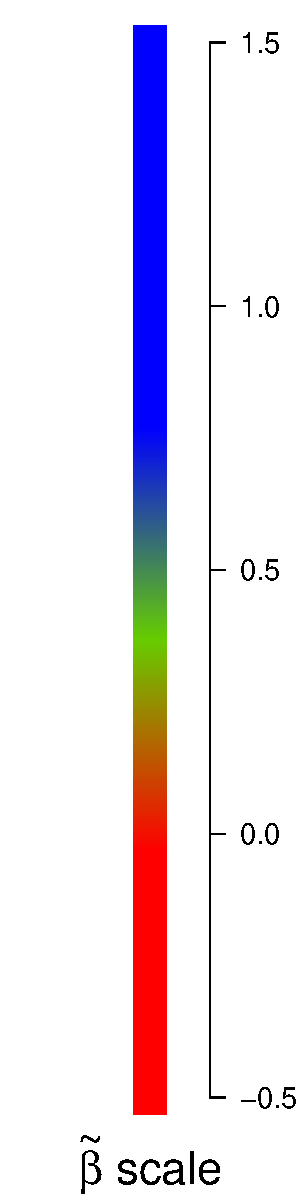
\includegraphics[width=1\linewidth]{betascale.pdf}
	\end{subfigure}
	\caption{The left hand side shows three plots of a historical thread with $d=1097$ and $v=1$, and the right hand side shows three plots of a manipulated thread with $d=1097$ and $v=9$. Top plots shows the log-ratio estimates over time (observation no.), with the geometric mean of the social information shown by a dotted line. Bottom left plots show the log-ratio of the estimates as a function of the log-ratio of the social information, indicating how differently participants use their social information. Bottom right plots show the cumulative distribution of individual $\tilde{\beta}$'s with 95\% intervals derived from the fitted models and added interquartile values of $\tilde{\beta}$.}
	\label{fig: social influence}
\end{figure*}

Figure \ref{fig: h d=1097, v=1} shows results for a historical thread where estimates are split among keepers (red), compromisers (green) and adopters (blue) throughout the thread. Figure \ref{fig: m d=1097, v=9} in contrast shows the results for a manipulated thread, where the same three groups are clearly visible, but the evolutionary trend is completely different compared to the historical thread. Contrasting Figures \ref{fig: h d=1097, v=1} and \ref{fig: m d=1097, v=9} clearly reveals different dynamics of threads in terms of manipulation or not. In general, our experiments show distinct distributions of overlapping groups (keepers, compromisers and adopters) in each thread, and in the case of manipulation suggest a substantial split into enthusiastic adopters versus skeptic keepers. The GMM framework is also applied to independent data from \cite{jayles2017social} allowing similar insights into qualitatively different tasks. 


\newpage

% Bibliography
\bibliographystyle{ci-format}
\bibliography{wamot}


\end{document}
